\documentclass{IEEEtran}
\def\BibTeX
\usepackage{cite}
\usepackage{url}
\usepackage{graphicx}
\graphicspath{ {./images/} }

%%%%%%%%%%%%%%%%%%%%
\begin{document}

\title{Extractive Summarization of BBC News Articles Using Na\"{i}ve Bayes and Frequency Driven Topic Representation}
\author{Parker Smith
\thanks{P. Smith is with the College of Computing and Software Engineering, Kennesaw State University, Marietta, GA, 30060 USA. Email: psmit216@students.kennesaw.edu}}

%%%%%%%%%%%%%%%%%%%%

\IEEEtitleabstractindextext{
    \begin{abstract}
    News is an essential part of the average American's life. From morning until evening, Americans ingest large quantities of different news topics. As the shift to a more digitized world ever increases, users can obtain their news from an increasing number of sources such as Newspapers, Radio, and Television. However, the most popular form of receiving news today is through Digital Media. The invention of digital media changed the news landscape forever and created new paths for all types of news outlets. Unfortunately, the generation of new media outlets lead to an excessive amount of text to read to understand the daily news: more so than someone can read in a day. An interesting solution to this problem is through text summarization. Instead of reading every article to learn important news, an algorithm can summarize the most important parts of the article to shorten a long, multi-paragraph article to a single easy to read paragraph. Current summarization models use multiple methods: Na\"{i}ve Bayes classifiers to identify ideal summary sentences based on a set of features, weighting sentences based on the summed TF-IDF score of the sentence, and many more not covered in this project. As one model by Kupiec, Pedersen, and Chen shows, a Na\"{i}ve Bayes classifier can produce an accurate summarization (defined as a summarization that would be produced by a professional) 84\% of the time \cite{related_naive_bayes_summarizer}. An additional baseline by Yih, Goodman, Vanderwende, and Suzuki shows that a TF-IDF summarization model can produce a summarization with a ROUGE-1 score of 0.374 \cite{related_tf-idf}. This project implements these two summarization models and compares their efficiencies and accuracies on a BBC News dataset. This dataset consists of 2,225 articles with an average of 18 sentences each that are split into multiple categories. The results from this project, evaluated using the ROUGE-2 $F_1$ Score metric, show that a Na\"{i}ve Bayes classifier can produce a summarization with an $F_1$ score of 0.5429 while a TF-IDF summarizer can produce a summarization with an $F_1$ score of 0.4302. Additionally, both models take less than 10 seconds to fully train.
    \end{abstract}
    \begin{IEEEkeywords}
    Text Summarization, Extractive Summarization, NLP, Na\"{i}ve Bayes, TF-IDF 
    \end{IEEEkeywords}
}

\maketitle
\IEEEdisplaynontitleabstractindextext

%%%%%%%%%%%%%%%%%%%%

\section{Introduction}
Studies have shown that "on a typical day, 92\% of Americans access news in multiple formats." \cite{news_reading_behavior} Before the creation of the Internet, news could only be gathered from hard-print and hand-distributed sources such as newspapers, or just from spoken word distribution. However, in the current age of technology, "people [are] increasingly [turning] to the Internet for daily news." \cite{news_reading_behavior} With the obvious shift to digital media and the ever-increasing number of news outlets available, it is difficult for someone to read all the news articles produced from their favorite news outlets.

This project is significant in that it summarizes long news articles to a few paragraphs, allowing a user to consume all the articles from their favorite news sources while drastically reducing the amount of reading required and reducing the time it takes to consume news. Three specific goals governed the creation of this project: summarize the news articles while retaining their original meaning, summarized articles should be shorter than the original, and a user should be able to learn the full content of the original article in a shorter period of time by reading the summarized article.

The primary application of this project is to make news articles easier for the average consumer to read. This allows more news topics to be available to all people because it will be quicker to read and understand a summarized news article. At that point, a user can read far more news topics in the same amount of time it would take them to read a single article. Ultimately, the goal of this project is to spread more knowledge by keeping all news readers up to date on a wide range of topics without them reading non-essential filler.

\section{Related Works}
\subsection{Deep Extractive Text Summarization \cite{related_work_1}}
This paper by R. Bhargava and Y. Sharma covers extractive summarization using deep learning techniques to summarize text. The primary model is a mixed Recurrent Neural Network (RNN) and Convolutional Neural Network (CNN). This was chosen because the CNN can quickly extract hidden features from the text by running it through convolution layers with kernels of different sizes. From there, the RNN can learn those features and select the sentences with the highest feature values. The dataset for this paper is Para Multiling 2015 which was designed for Multilingual Single-document Summarization. Each document contains both the raw text and a human generated summary for testing evaluation. The important performance metrics for this model are Training Accuracy, Testing Accuracy, Testing Precision, Testing Recall, and Testing F-Score. The results have the model with a Training Accuracy of 96.15\%, a Testing Accuracy of 75.70\%, a Testing Precision of 0.2500, a Testing Recall of 0.4287, and a Testing F-Score of 0.3157. Some limitations to this paper include a lack of detailed information on the dataset and a weak idea of how the proposed summarization approach is implemented. No statistical information is given on the dataset such as the number of sentences, number of documents, or vocabulary size of the dataset. Additionally, the proposed summarization approach claims to divide the model into two phases, yet no implementation or discussion of those two phases are shown. The methodology proposed by Bhargava and Sharma is quite different from this project's. However, it provides a good baseline as another implementation method of extractive text summarization.

\subsection{Extractive Hotel Review Summarization based on TF/IDF and Adjective-Noun Pairing by Considering Annual Sentiment Trends \cite{related_work_2}}
In another paper by G. N. H., R. Siautama, A. C. I. A., and D. Suhartono, hotel reviews are summarized in an attempt to simplify the process of sentiment analysis. Instead of finding the sentiment of long, exhaustive reviews, the review is summarized and the sentiment of the entire review is based off the sentiment of the summarized review. For this paper, extractive summarization is implemented with Term Frequency Inverse Document Frequency (TF-IDF) as the primary summarization method. No specific algorithm was designed for their model, however a generic TF-IDF algorithm was used to score sentences, and preprocessing was implemented through sentence segmentation, case folding, and tokenization. The dataset used for this paper is a list of hotel reviews scraped from TripAdviser.com. There are a total of 21,746 reviews, 1,370 of which contain text from a total of 167 different hotels. The performance metrics for this paper are the ROUGE and BLEU evaluation methods. The average ROUGE recall is 0.1200, the average ROUGE precision is 0.1917, and the BLEU precision is 0.4443. A major limitation of this paper is a complete lack of information on how the paper’s authors implement the algorithms. No information is given on how the TF-IDF score is generated and how the sentences are scored. The methodology implemented by H., Siautama, A., and Suhartono is similar to this project's methodology in that both employ TF-IDF as one of the primary ways of scoring sentences. However, there could be differences in how both TF-IDF algorithms are implemented. Unfortunately, it is impossible to know as this paper does not showcase their algorithm.

\section{Methodology}
In general there are two primary forms of text summarization: Extractive Summarization and Abstractive Summarization \cite{related_summarization}.  "Purely extractive summaries often times give better results compared to automatic abstractive summaries," \cite{related_summarization} therefore this project will solely focus on Extractive Summarization. This technique produces summaries by "choosing a subset of the sentences in the original text." \cite{related_summarization} Typically, the sentences with the greatest importance are singled out and combined together to create the final summarized article. \cite{related_summarization}

There are multiple ways of implementing Extractive Summarization, however all of them follow three primary tasks: constructing intermediate representations of the text, scoring the intermediate representations based on how well they represent the topic, and selecting a certain number of sentences to represent the final, summarized text \cite{related_summarization}. Typically, vectors are constructed as the intermediate text representations. However, there is another method we will also use in this project called topic representation, which does not identify sentences by their features, but instead attempts to directly interpret the topics found within the text \cite{related_summarization}. Once intermediate representations are generated, they are scored by a numeric value determining how well the sentence describes the content of the text. This could be implemented through a frequency count or a relational count. Finally, the selected summarization sentences are reconstructed to their original text and combined to create the fully summarized article.

This project will compare two separate methodologies that implement Extractive Summarization in order to ascertain which method performs with the highest efficiency. The first method implements a frequency driven approach of topic representation as a way to construct intermediate representations of the text. This is accomplished through Term Frequency Inverse Document Frequency (TF-IDF) \cite{tf-idf}. TF-IDF is comprised of two parts: Term Frequency and Inverse Document Frequency. The Term Frequency identifies the number of times the given term appears in the document. Its formula is 
\[tf(t, D) = \frac{count(t)}{length(D)}\]
where t is the term and D is the set of documents. The Inverse Document Frequency "looks at how common (or uncommon) a word is [among the documents]." \cite{tf-idf} Its formula is
\[idf(t, D, N) = log(\frac{N}{count(d \in D:t \in d)})\]
where t is the term, D is the set of documents, and N is the number of documents in the set of documents. The TF-IDF value is then found by multiplying these two values together. This determines the importance of each term, reducing the importance if the term is found often in every document. This decreases the importance of commonly occuring words such as "is" and "the." Once the intermediate representation of the text has been generated, the sentences are scored by summing the vectors within the sentences. Finally, the n-highest scored sentences are chosen as the sentences to summarize the full article. This is visually displayed in Figure \ref{fig:tfidf_diagram}.

\begin{figure}[h]
\centering
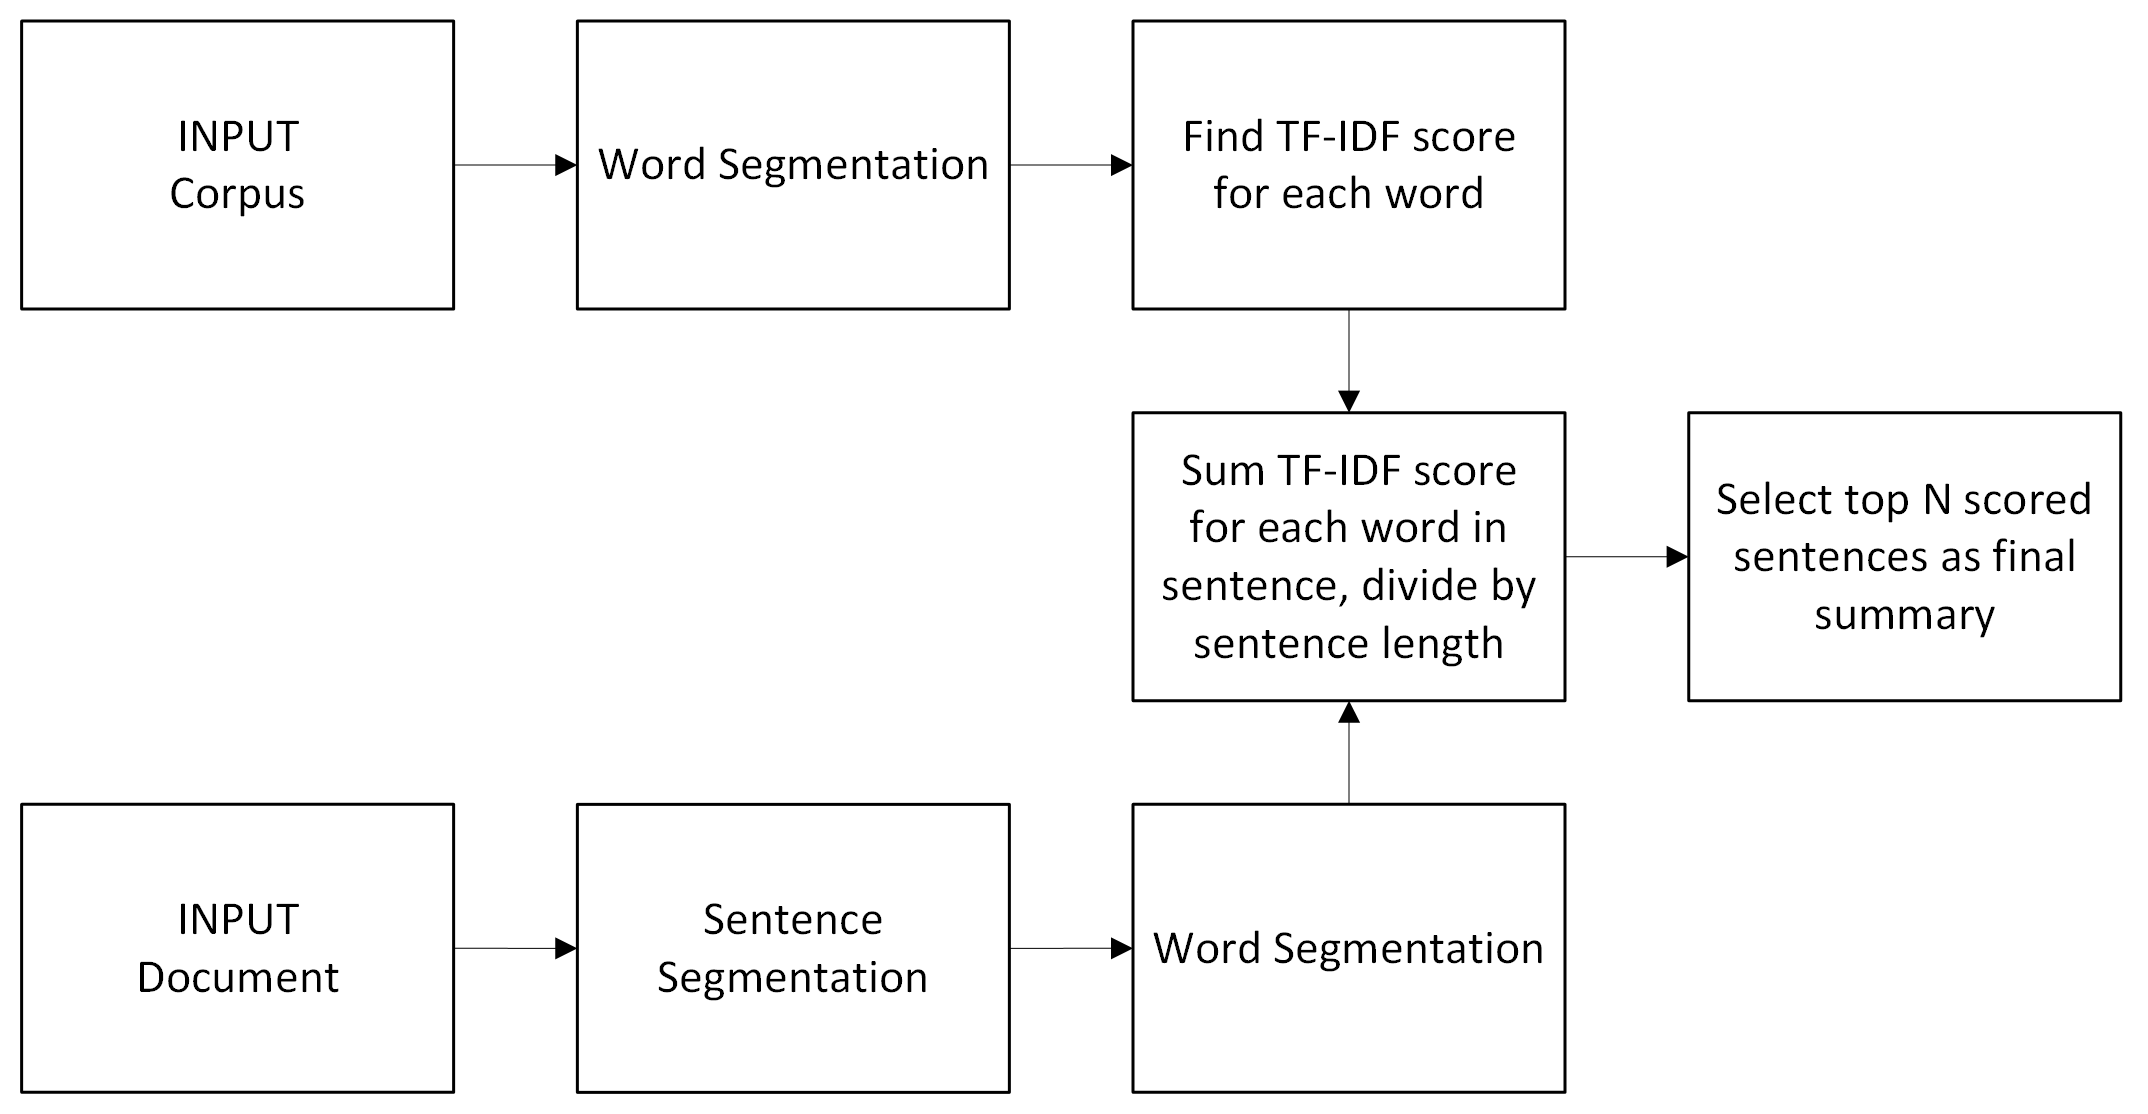
\includegraphics[width=0.475\textwidth]{images/TF-IDF_Diagram.png}
\caption{High-Level Architectural Diagram for the TF-IDF Summarizer}
\label{fig:tfidf_diagram}
\end{figure}

The second method this project will use implements the indicator representation approach of intermediate representation. Instead of attempting to score the sentences by topic, "Indicator representation approaches describe every sentence as a list of features (indicators) of importance such as sentence length, position in the document, having certain phrases, etc" \cite{related_summarization}. This project will perform this type of representation using a Na\"{i}ve Bayes Machine Learning classifier. Na\"{i}ve Bayes classifiers function off of the Bayes Rule:
\[P(s \in S | F_1, F_2, ...F_k) = \frac{P(F_1, F_2, ...F_k | s \in S)P(s \in S)}{P(F_1, F_2, ...F_k)}\]
\cite{related_naive_bayes_summarizer}. Assuming that all sentences are statistically independent, the classifier can be summarized as
\[P(s \in S | F_1, F_2, ...F_k) = \frac{\Pi_{j=1}^k P(F_j | s \in S)P(s \in S)}{\Pi_{j=1}^k P(F_j)}\]
\cite{related_naive_bayes_summarizer}. Since all parts of the function are constant or can be found directly from the training set, this function can directly output a probability of how applicable each sentence is to be selected for the summarization \cite{related_naive_bayes_summarizer}. Once probabilities are assigned to all sentences, the sentences with the n-highest probabilities are selected to summarize the article. The high-level diagram for this process is shown in Figure \ref{fig:naive_bayes_diagram}.

\begin{figure}[h]
\centering
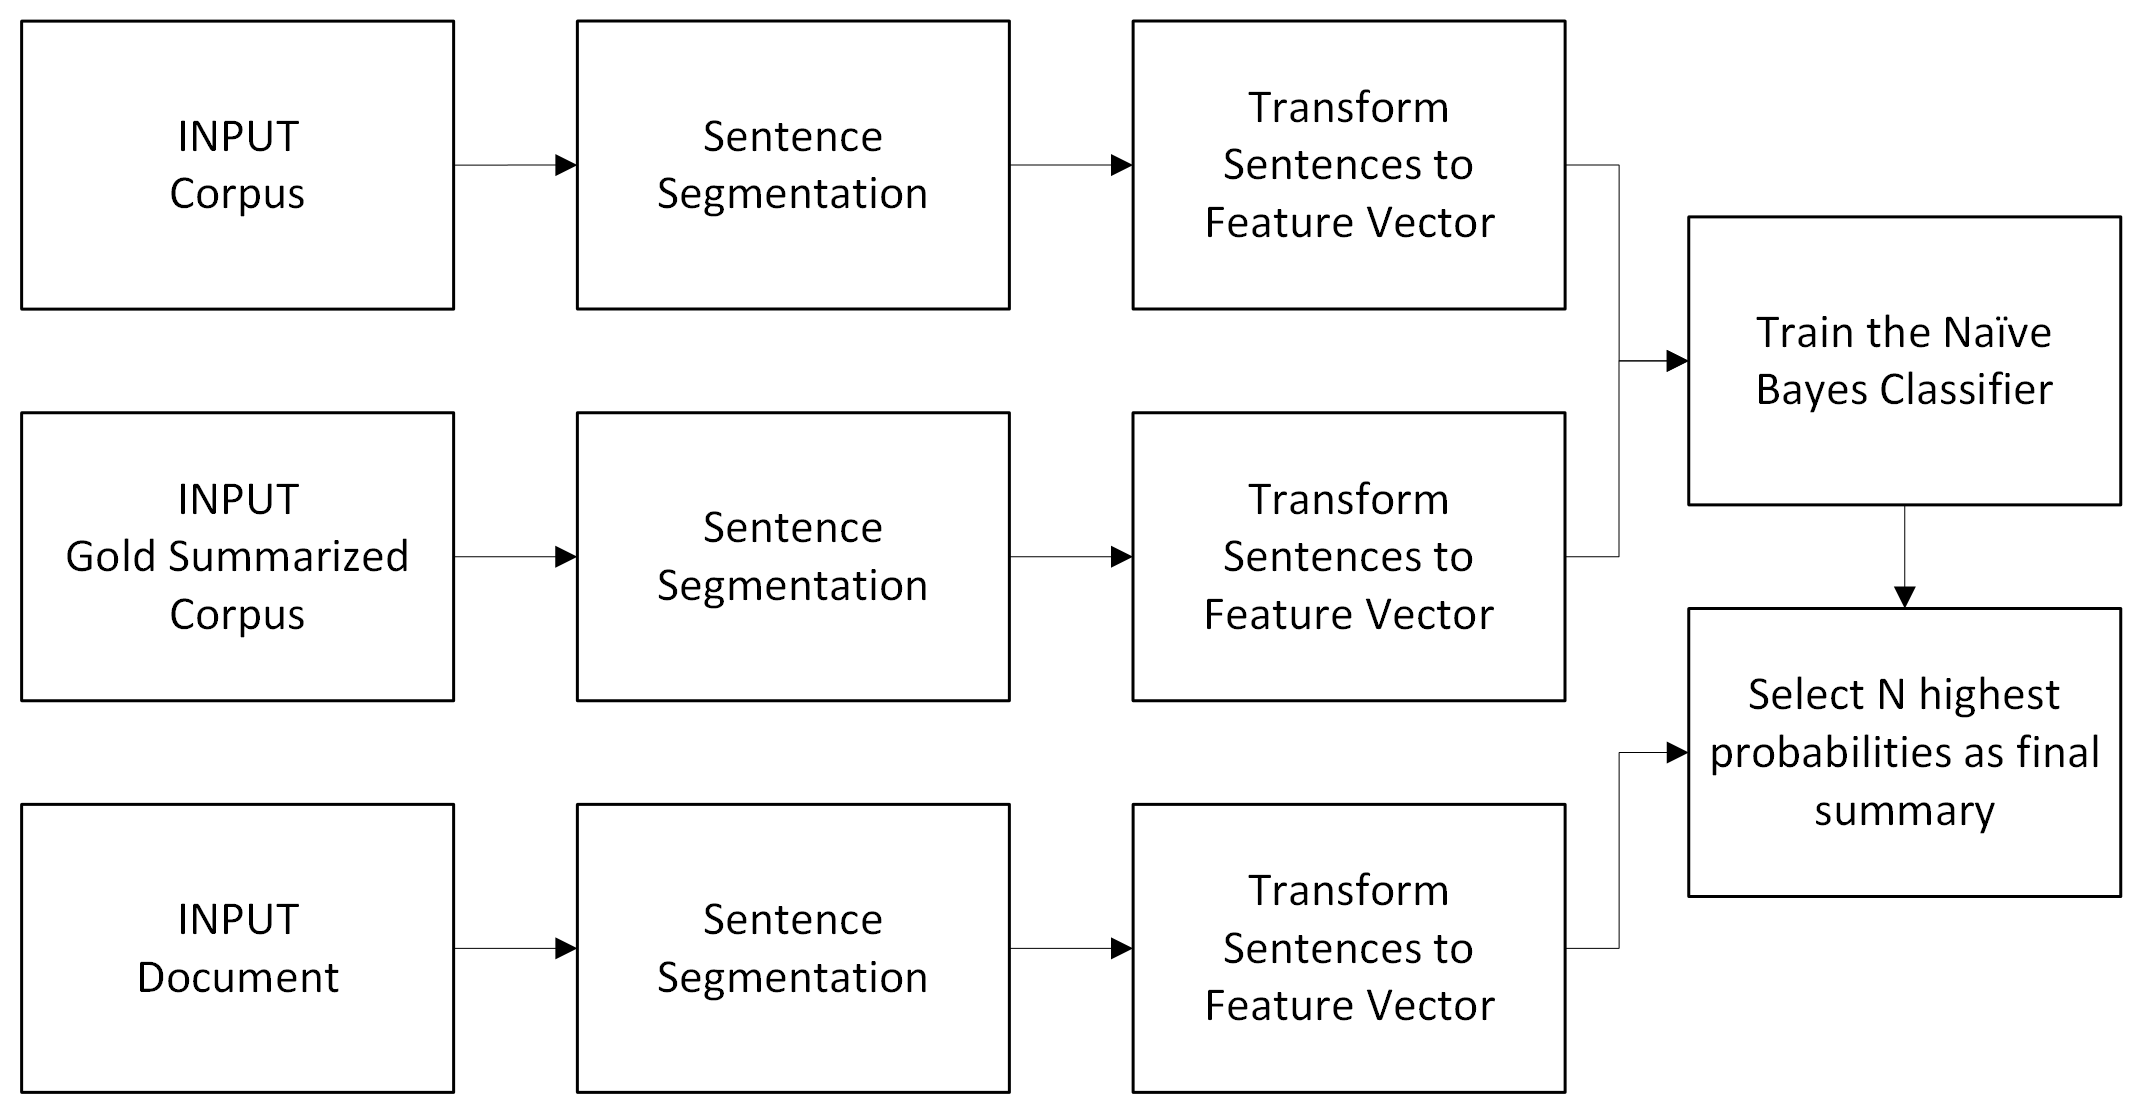
\includegraphics[width=0.475\textwidth]{images/NaiveBayes_Diagram.png}
\caption{High-Level Architectural Diagram for the Na\"{i}ve Bayes Summarizer}
\label{fig:naive_bayes_diagram}
\end{figure}

\section{Experimental Setup}
The dataset for this project is a set of articles from BBC News obtained from Kaggle \cite{dataset}. The article's topics include business, entertainment, politics, sports, and technology. The entire dataset includes 2,225 articles as summarized in Table \ref{table:dataset_article_count}.

\begin{table}[h]
\centering
\caption{Number of articles contained within the dataset}
\begin{tabular}{|l|l|l|l|l|l|}
\hline
Business & Entertainment & Politics & Sports & Technology & Total \\ \hline
510 & 386 & 417 & 511 & 401 & 2225 \\ \hline
\end{tabular}
\label{table:dataset_article_count}
\end{table}

Conveniently, the dataset includes both raw articles and final summarized articles that can be used by the Na\"{i}ve Bayes classifier to determine the features of a sentence chosen for summarization. In addition, a 10\% testing-training split will be used, therefore 2,002 articles will go towards training and 223 articles will go towards testing. Table \ref{table:dataset_summary} showcases the number of sentences, number of tokens, and the total vocabulary size of the dataset.

\begin{table}[h]
\centering
\caption{Summary of the dataset's lexical features, sorted by category}
\begin{tabular}{|l|l|l|l|}
\hline
Category    &Sentences  &Tokens     &Vocabulary Size \\ \hline
Business    &8,016      &169,762    &97,366 \\ \hline
Entertainment&6,157     &128,700    &72,695 \\ \hline
Politics    &8,642      &190,809    &99,455 \\ \hline
Sports      &8,642      &170,019    &96,565 \\ \hline
Technology  &9,661      &203,212    &102,883 \\ \hline
Total       &41,118     &862,502    &468,964 \\ \hline
\end{tabular}
\label{table:dataset_summary}
\end{table}

All code for this project is implemented in Python and uses scikit-learn's TfidfVectorizer \cite{scikit-learn_tf-idf} as the base for the TF-IDF summarizer and scikit-learn's CategoricalNB \cite{scikit-learn_naive_bayes} as the base for the Na\"{i}ve Bayes summarizer. The other important package used for data manipulation is NumPy \cite{numpy}. All models were tested on a personal computer running Windows 10 with 8 GB of RAM and a 2.10 GHz processor. 

\section{Implementation Details}
In order to correctly implement the TF-IDF vectorizer and the Na\"{i}ve Bayes classifier, all documents read from the dataset had to be tokenized. The two forms of tokenization applied were sentence tokenization and word tokenization. All tokenization was implemented through regular expressions. The regular expression for sentence tokenization is
\begin{verbatim}
[^ \n].+?\.(?!\d)
\end{verbatim}
while the regular expression for word tokenization is
\begin{verbatim}
\S?\d+[.,]\d+\w+|[^ \n,.]+
\end{verbatim}

The TF-IDF Summarizer has the scikit-learn TfidvVectorizer \cite{scikit-learn_tf-idf} as its base. Scoring is implemented by enumerating through each word in the sentence and summing the vector score for each word within the sentence. The resulting score is divided by the word count of the sentence to eliminate bias caused by longer sentences. The sentences with the top N scores are then selected as the summary sentences.

The Na\"{i}ve Bayes Summarizer is built upon the scikit-learn CategoricalNB \cite{scikit-learn_naive_bayes} classifier. It requires each sentence to be vectorized to a set of handcrafted features. Those features are Sentence Length, Location within the Paragraph, Similarity to the Title, and whether or not the sentence contains a significant amount of words with uppercase letters. Each feature and their categorical splits are shown in Table \ref{table:nb_features}.

\begin{table}[h]
\centering
\caption{Na\"{i}ve Bayes Classifier's Features}
\begin{tabular}{|l|l|l|l|}
\hline
Feature  & \multicolumn{3}{|c|}{Splits} \\ \hline
Sentence Length  & \verb|<|12  & 12-25  & \verb|>|25 \\ \hline
Pargraph Location  & Beginning  & Middle  & End \\ \hline
Title Similarity  & Non-Similar  & Similar  & \\ \hline
Has Uppercase  & \verb|>|1 Uppercase Word  & No Uppercase & \\ \hline
\end{tabular}
\label{table:nb_features}
\end{table}

Once the sentences are vectorized, the model is trained against some gold-standard human-summarized articles. After training, the document to be summarized is run through the summarizer and each sentence's log probability of being in the final summary is calculated. The top N scoring sentences are selected as the final summary sentences.

\section{Results}
For each model, this project calculated the recall, precision, and F1 score for the ROUGE-1, ROUGE-2, and ROUGE-3 metrics. The training time of each model was also logged. These results, along with those from the related works, are shown in Table \ref{table:results_comparison}.

\begin{table}[h]
\raggedleft
\caption{Results for This Project's Models and some Baseline Models}
\begin{tabular}{|lcccc|}
\hline
\multicolumn{1}{|l|}{}              & \multicolumn{2}{c|}{This Project}                                 & \multicolumn{1}{c|}{Related 1}    & Related 2 \\ \hline
\multicolumn{1}{|l|}{Model Name}    & \multicolumn{1}{c|}{Na\"{i}ve Bayes} & \multicolumn{1}{c|}{TF-IDF}    & \multicolumn{1}{c|}{Deep NN} & TF-IDF         \\ \hline
\multicolumn{5}{|l|}{\textbf{ROUGE-1}}                                                                                                                            \\ \hline
\multicolumn{1}{|l|}{Recall}        & \multicolumn{1}{c|}{0.4542}      & \multicolumn{1}{c|}{0.3782}    & \multicolumn{1}{c|}{0.4287}            & 0.1686         \\ \hline
\multicolumn{1}{|l|}{Precision}     & \multicolumn{1}{c|}{0.4726}      & \multicolumn{1}{c|}{0.4251}    & \multicolumn{1}{c|}{0.2500}            & 0.2885         \\ \hline
\multicolumn{1}{|l|}{$F_1$ Score}    & \multicolumn{1}{c|}{0.4632}      & \multicolumn{1}{c|}{0.4003}    & \multicolumn{1}{c|}{0.3157}            & 0.2057         \\ \hline
\multicolumn{5}{|l|}{\textbf{ROUGE-2}}                                                                                                                            \\ \hline
\multicolumn{1}{|l|}{Recall}        & \multicolumn{1}{c|}{0.5305}      & \multicolumn{1}{c|}{0.4091}    & \multicolumn{1}{c|}{-}                 & 0.0239         \\ \hline
\multicolumn{1}{|l|}{Precision}     & \multicolumn{1}{c|}{0.5559}      & \multicolumn{1}{c|}{0.4537}    & \multicolumn{1}{c|}{-}                 & 0.0355         \\ \hline
\multicolumn{1}{|l|}{$F_1$ Score}    & \multicolumn{1}{c|}{0.5429}      & \multicolumn{1}{c|}{0.4302}    & \multicolumn{1}{c|}{-}                 & 0.0282         \\ \hline
\multicolumn{5}{|l|}{\textbf{ROUGE-3}}                                                                                                                            \\ \hline
\multicolumn{1}{|l|}{Recall}        & \multicolumn{1}{c|}{0.5222}      & \multicolumn{1}{c|}{0.3970}    & \multicolumn{1}{c|}{-}                 & -              \\ \hline
\multicolumn{1}{|l|}{Precision}     & \multicolumn{1}{c|}{0.5463}      & \multicolumn{1}{c|}{0.4373}    & \multicolumn{1}{c|}{-}                 & -              \\ \hline
\multicolumn{1}{|l|}{$F_1$ Score}    & \multicolumn{1}{c|}{0.5340}      & \multicolumn{1}{c|}{0.4162}    & \multicolumn{1}{c|}{-}                 & -              \\ \hline
\multicolumn{1}{|l|}{Training Time} & \multicolumn{1}{c|}{8.18 secs}   & \multicolumn{1}{c|}{1.53 secs} & \multicolumn{1}{c|}{-}                 & -              \\ \hline
\end{tabular}
\label{table:results_comparison}
\end{table}

Table \ref{table:results_comparison} shows that when comparing the ROUGE-1 metric, this project's models perform much better than those from the related works. There is at least a 10\% difference in $F_1$ Score between the related works' models and this project's models. When comparing the two models created in this project, both have highly similar scores, with the Na\"{i}ve Bayes slightly pulling out ahead when all $F_1$ scores from all ROUGE metrics are compared. However, the Na\"{i}ve Bayes summarizer does take slightly longer to train and does require a gold-standard of pre-summarized articles to train with.

Quotation \ref{quotation:non-summarized} displays an unsummarized article from the corpus. Quotation \ref{quotation:tfidf-summarized} and quotation \ref{quotation:nb-summarized} display the summarized version of the article from the TF-IDF Summarizer and the Na\"{i}ve Bayes Summarizer respectively. 

\subsection{Full Article from the Corpus}
\begin{quotation}
Tate \& Lyle boss bags top award

Tate \& Lyle's chief executive has been named European Businessman of the Year by a leading business magazine.

Iain Ferguson was awarded the title by US publication Forbes for returning one of the UK's "venerable" manufacturers to the country's top 100 companies. The sugar group had been absent from the FTSE 100 for seven years until Mr Ferguson helped it return to growth. Tate's shares have leapt 55\% this year, boosted by firming sugar prices and sales of its artificial sweeteners.

"After years of a sagging stock price and a seven-year hiatus from the FTSE 100, one of Britain's venerable manufacturers has returned to the vaunted index," Forbes said. Mr Ferguson took the helm at the company in 2003, after spending most of his career at consumer goods giant Unilever. Tate \& Lyle, which was an original member of the historic FT-30 index in 1935, operates more than 41 factories and 20 more additional production facilities in 28 countries. Previous winners of the Forbes award include Royal Bank of Scotland chief executive Fred Goodwin and former Vodafone boss Chris Gent.
\label{quotation:non-summarized}
\end{quotation}

\subsection{Article Summarized using This Project's TF-IDF Summarizer}
\begin{quotation}
Tate \& Lyle boss bags top award

Iain Ferguson was awarded the title by US publication Forbes for returning one of the UK's "venerable" manufacturers to the country's top 100 companies. The sugar group had been absent from the FTSE 100 for seven years until Mr Ferguson helped it return to growth. Tate's shares have leapt 55\% this year, boosted by firming sugar prices and sales of its artificial sweeteners. "After years of a sagging stock price and a seven-year hiatus from the FTSE 100, one of Britain's venerable manufacturers has returned to the vaunted index," Forbes said. Mr Ferguson took the helm at the company in 2003, after spending most of his career at consumer goods giant Unilever. Previous winners of the Forbes award include Royal Bank of Scotland chief executive Fred Goodwin and former Vodafone boss Chris Gent.
\label{quotation:tfidf-summarized}
\end{quotation}

\subsection{Article Summarized using This Project's Na\"{i}ve Bayes Summarizer}
\begin{quotation}
Tate \& Lyle boss bags top award

Tate \& Lyle's chief executive has been named European Businessman of the Year by a leading business magazine. Iain Ferguson was awarded the title by US publication Forbes for returning one of the UK's "venerable" manufacturers to the country's top 100 companies. The sugar group had been absent from the FTSE 100 for seven years until Mr Ferguson helped it return to growth. "After years of a sagging stock price and a seven-year hiatus from the FTSE 100, one of Britain's venerable manufacturers has returned to the vaunted index," Forbes said. Mr Ferguson took the helm at the company in 2003, after spending most of his career at consumer goods giant Unilever. Tate \& Lyle, which was an original member of the historic FT-30 index in 1935, operates more than 41 factories and 20 more additional production facilities in 28 countries.
\label{quotation:nb-summarized}
\end{quotation}

\section{Discussion and Conclusion}
This project proves that it is possible to create effective summaries using both supervised and unsupervised extractive methods. Both models returned results that provided a summary that could be read and understood by a human. The primary challenges to these methods, and all summarization methods, is that it is almost impossible to define a "good summary." Human-based evaluation methods are highly accurate, but are incredibly labor and time intensive. Therefore, automatic evaluation methods such as ROUGE must be used. A future improvement to these models would be to attempt to find a more accurate way of determining how "good" a summary is when compared to either a human-generated gold-standard summary or the non-summarized document. Another improvement that could be made would be to add more features to the Na\"{i}ve Bayes classifier. These new features would provide an extra level of flexibility to the model and would allow it to further refine which sentences appear in summaries most often. In conclusion, extractive summarization, both supervised and unsupervised, is highly feasible. The summaries are easy to read, provide a good amount of information to the reader, and allow them to read more news articles in a shorter period of time.

%%%%%%%%%%%%%%%%%%%%

\bibliographystyle{IEEEtran}
\bibliography{References}

%%%%%%%%%%%%%%%%%%%%

\end{document}